\chapter{Theory}


\section{Wave Theory}

Simple Wave Theory

\section{Energy Spectra}

\subsection{Phillips Spectrum}
\subsection{Mobley Spectrum}
\subsection{SWAP}
\subsection{JONSWAP}


Energy Spectrum

$\int x(t) dt$

$k=\frac{\pi}{\mathbf y}$

\begin{equation}\label{eq:test} x = y \end{equation}

We can give an equation a label so that we can refer to it later.
\begin{equation}
\label{eq:ising}
E = -J \sum_{i=1}^N s_i s_{i+1} ,
\end{equation}
Equation~\eqref{eq:ising} expresses the energy of a configuration
of spins in the Ising model.

\section{The Rendering Pipeline}
The rendering pipeline constitutes the core of real-time graphics. It's task
consists in generating, or rendering, a two-dimensional output image given a
virtual camera, scene geometry, materials and
lightsources\cite{book:akenine-rtr}. As shown in Figure~\ref{fig:RAGR} the
rendering pipeline can be divided into three conceptual stages:
\begin{itemize}
 \item The \textit{application stage} holds all necessary information to break
down the scene geometry into smaller chunks which actually are passed on to the
geometry stage.
 \item The \textit{geometry stage} transforms the input geometry to a
two-dimensional output coordinate system.
 \item The \textit{rasterizer stage} fills the primitives output by the
geometry stage with color.
\end{itemize}

\begin{figure}
\begin{center}
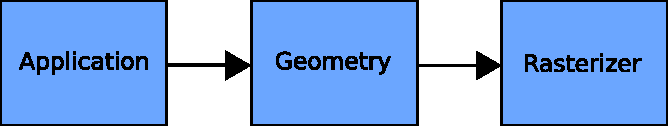
\includegraphics[scale=0.8]{Images/Rendering-Pipeline-AGR.pdf}
\caption{The three stages of the rendering pipeline.}
\label{fig:RAGR}
\end{center}
\end{figure}

\subsection{Application Stage}
The application stage implements the whole program logic. It's structure and
implementation is entirely dependent on the the task it should perform. One
such a task could be a simple triangle mesh visualisation, another, more
complex one, a complete 3D computer game. What these tasks have in common, is
that all of them require the application stage to provide the geometry stage
with appropriately prepared data for further processing.

Usually the application stage's main task is broken down into three subtasks:
\begin{itemize}
 \item Take \textit{user input}
 \item \textit{Update} the internal state
 \item \textit{Render} by feeding data to the next stage
\end{itemize}

A common task which resides in the application stage is \textit{collision
detection and response}: to detect if two objects collide and update their
internal state accordingly. Nowadays this is often done by a physics library,
such as \textit{NVIDIA PhysX}\cite{misc:ageia-physx} or \textit{Havok
Physics}\cite{misc:havok}.

In the case the application stage deals with large amounts of geometric
objects in a scene, it may prove necessary to reduce the amount of data which
is sent to the geometry stage. This is done by discarding objects invisible to
the viewer before they are actually handed over to the geometry stage,
effectively reducing the geometry stage's workload.

Whereas the geometry and rasterizer stages are to be found on the graphics
hardware, the application stage is typically executed in software on the CPU;
known exceptions are e.g. hardware accelerated physics and sound.

\subsection{Geometry Stage}

\begin{figure}
\begin{center}
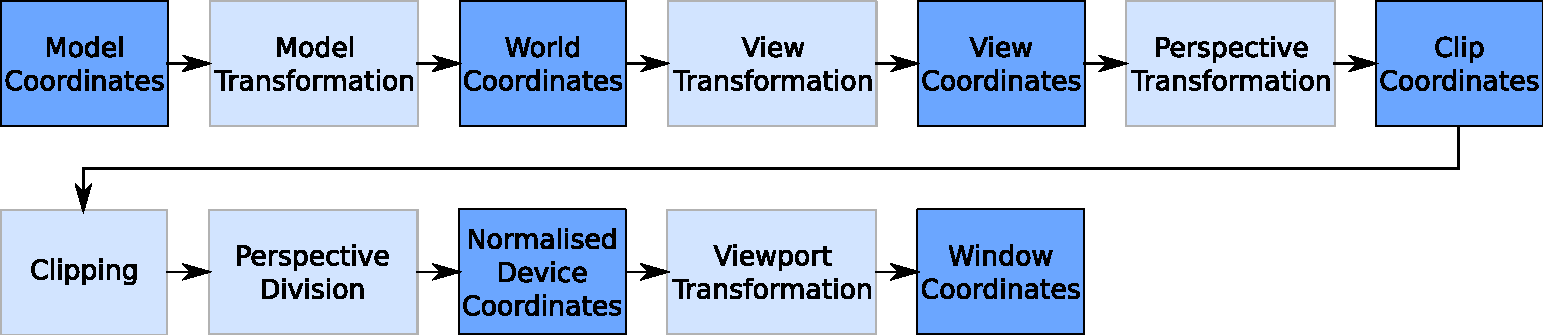
\includegraphics[scale=0.5]{Images/Geometry-Stage.pdf}
\caption{The Geometry stage.}
\label{fig:GeometryStage}
\end{center}
\end{figure}

The geometry stage takes geometric primitives as input from the application
stage and processes them, so that the next stage, the rasterizer stage, may
calculate the final color for a pixel or fragment. Figure
\ref{fig:GeometryStage} shows all coordinate systems and operations involved. In
order to do that, the geometric primitives have to be \textit{transformed}
through several \textit{coordinate systems}, eventually reaching the
\textit{image space}. Transformations, such as rotation, translation,
scaling and shearing, usually are represented by matrices. For a
three-dimensional space 4x4 matrices are needed to be able to specify the
aforementioned transformations. In addition those transformations can be
concatenated by multiplying the matrices together, thereby reducing the
arithmetic workload to compute multiple transformations.
The geometry stage can be broken up in two larger parts:
\begin{itemize}
 \item  the model-view stage, which is concerned with the setup of a scene by
positioning different models and the camera
 \item the projection stage, which has to depict the assembled scene onto the
image plane
\end{itemize}

\subsubsection{The Model-View Transformation}

The \textit{model space} serves as starting point, as each model resides
therein, simply meaning that no transformation has been applied to the model
coordinates. By orienting and positioning such a model in the world, it gets
transformed to \textit{world space}. There may be more instances of the same
model in the world, possibly differing in orientation and position. The world
space itself is unique, all models are transformed with their respective model
transform and thereafter all are located in the world space. The next
coordinate system in the pipeline is the \textit{view space}, also known as
\textit{eye space}, which represents all objects or models in the world relative
to the camera. The camera itself is able to capture only a part of the world,
depending on the camera's position, viewing direction, field of view and viewing
range. The subvolume of the world the camera is actually able to see is called
the \textit{view frustum}. Figure~\ref{fig:ModelWorldView} shows the
steps from model to view space in a simplified manner.

\begin{figure}[t]
\centering
\subfigure[Model Space]
{
  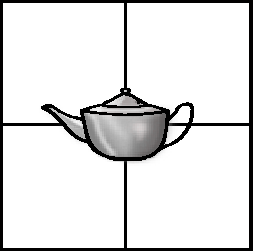
\includegraphics[scale=0.7]{Images/ModelSpace.pdf}
  \label{fig:subfigmodelspace}
}
\subfigure[World Space]
{
  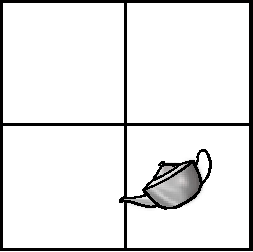
\includegraphics[scale=0.7]{Images/WorldSpace.pdf}
  \label{fig:subfigworldspace}
}
\subfigure[Camera Frustum]
{
  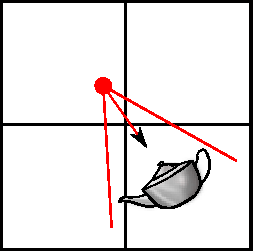
\includegraphics[scale=0.7]{Images/WorldSpaceWithCamera.pdf}
  \label{fig:subfigworldspacewithcamera}
}
\subfigure[View Space]
{
  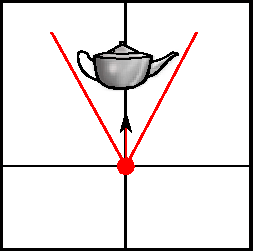
\includegraphics[scale=0.7]{Images/ViewSpace.pdf}
  \label{fig:subfigviewspace}
}
\caption[Model, World and View space]{Starting point is the model
space~\subref{fig:subfigmodelspace}, next our sample model ist rotated and
positioned in the world \subref{fig:subfigworldspace}. Since we want to view the
scene from within world space we add an observing camera
\subref{fig:subfigworldspacewithcamera}. The view frustum is highlighted in
red. At last, \subref{fig:subfigviewspace} shows the world relative to the
camera.}
\label{fig:ModelWorldView}
\end{figure}

\subsubsection{The Projection}

The projection's task is to transform objects or models from three-dimensional
view space onto a two-dimensional image plane. On current graphics hardware the
task at hand consists of four steps in the following order:
\begin{itemize}
 \item the \textit{projection}
 \item \textit{viewport clipping}
 \item the \textit{perspective division}
 \item the \textit{viewport transform}
\end{itemize}

The projection in combination with the perspective division transforms
coordinates from view space into \textit{normalised device coordinates},
\textit{NDC} in short. NDC lie in a space called \textit{the canonical view
volume}, see Figure~\ref{fig:canonicalviewvolume}. The target volume is
represented by a cube, but the shape of the source volume, meaning the view
frustum, depends on the actual projection. Figure~\ref{fig:viewfrustum3d} shows
a possible view frustum in detail. There are a couple of different projections
to be found in computer graphics, the two most common types are the
\textit{parallel projection} and the \textit{perspective projection}.
Figure~\ref{fig:projections2d} illustrates their working principle,
Figure~\ref{fig:parallelandperspectivefrustum} shows their associated view
frusta. In short, the projection in combination with the perspective division
warps the view frustum into a cube.

\begin{figure}
\begin{center}
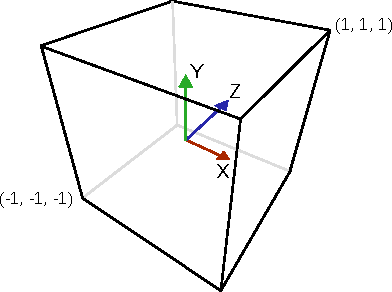
\includegraphics[scale=0.8]{Images/CanonicalCube.pdf}
\caption{The canonical view volume ranging from lower left (-1, -1, -1) to
uppper right (1, 1, 1). As opposed to the model, world and view space,
normalised device coordinates are lefthanded, with the positive z axis
pointing away from the viewer. The nearplane lies at z = -1, the far plane at z
= 1.}
\label{fig:canonicalviewvolume}
\end{center}
\end{figure}

\begin{figure}
\begin{center}
 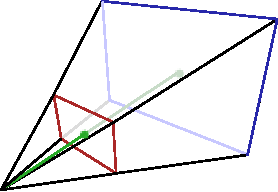
\includegraphics[scale=1.0]{Images/Frustum.pdf}
 \caption{The far plane, which represents the camera's viewing range is shown
in blue. The near plane, which is the plane where the objects in the scene get
projected onto, is highlighted in red. The green line depicts the viewing
direction, intersecting the center of the near and far plane.}
 \label{fig:viewfrustum3d}
\end{center} 
\end{figure}

\begin{figure}
\centering
\subfigure[Parallel Projection]
{
  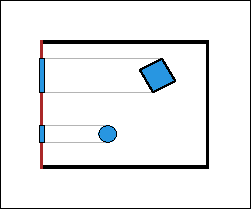
\includegraphics[scale=1.1]{Images/ParallelProjection2D.pdf}
  \label{fig:subfigparallelprojection2d}
}
\subfigure[Perspective Projection]
{
  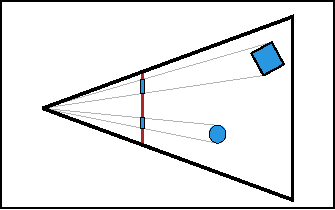
\includegraphics[scale=1.1]{Images/PerspectiveProjection2D.pdf}
  \label{fig:subfigperspectiveprojection2d}
}
\caption[View frustum, canonical cube]{Parallel lines are still parallel
after parallel projection~\subref{fig:subfigparallelprojection2d}, but not
after perspective projection~\subref{fig:subfigperspectiveprojection2d}.
The key property of the perspective projection is that objects that lie
farther away are depicted smaller than objects which lie near the image plane.}
\label{fig:projections2d}
\end{figure}

\begin{figure}
\centering
\subfigure[Parallel frustum]
{
  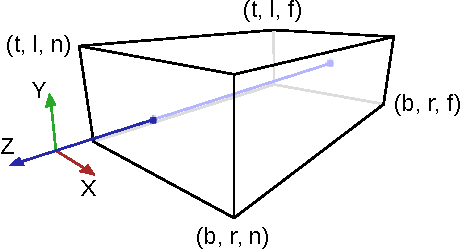
\includegraphics[scale=0.8]{Images/ParallelFrustum.pdf}
  \label{fig:subfigorthofrustum}
}
\subfigure[Perspective frustum]
{
  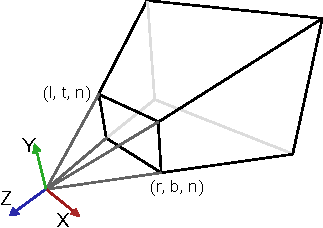
\includegraphics[scale=0.8]{Images/PerspectiveFrustum.pdf}
  \label{fig:subfigperspectivefrustum}
}
\caption[Parallel and Perspective Frustum]{The parallel frustum shown
in~\subref{fig:subfigorthofrustum} is a rectangular box, the perspective 
frustum in \subref{fig:subfigperspectivefrustum} resembles a truncated
pyramid. The paramters \textit{n} and \textit{f} stand for the distance from the
camera to the near and far plane. \textit{t}, \textit{b}, \textit{l} and
\textit{r} are derived from the camera's field of view as well as the image
plane's aspect ratio.}
\label{fig:parallelandperspectivefrustum}
\end{figure}

What happens to objects outside or partially inside the view frustum, though?
Clipping does take care of such primitives - it removes all primitives which
lie outside the view frustum and clips those which are partially inside to the
frustum's border. This way only primitives inside the canonical view volume are
passed on to the rasterizer stage, thus minimising it's workload. Clipping is
done in \textit{clip space}, right after the projection, but before the
perspective division. As mentioned before, after the perspective division
coordinates are in NDC, but they are still not related to the output window,
which is what the user actually will be able to see on the output device. The
viewport transform is the missing piece, it takes NDC as input, discards the
depth coordinate, and transforms the remaining two-dimensional coordinates to
window coordinates using the size and origin of the current viewport as
parameters.

\subsection{Rasterizer Stage}

triangle setup
scan conversion and interpolation
per fragment operations (texturing, ummadumshadern)
alpha test
depth test
stencil test
\begin{figure}[h]
\begin{center}
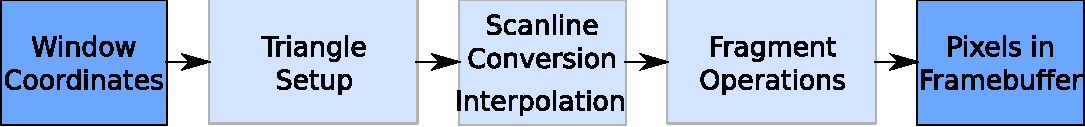
\includegraphics[scale=0.5]{Images/Rasterizer-Stage.pdf}
\caption{The Rasterizer stage.}
\label{fig:RasterizerStage}
\end{center}
\end{figure}

\section{The Projected Grid}

postprojection coordinates transformed to worldspace
grid on near and far plane, intersection with the y=0 plane
decouple projector from camera

\subsection{The Projector}
positioning
rotating
original is a hack, persistent grid mapping has a more stable approach
not optimal, because of "popping" at great distances
not so optimal distribution of the mesh resolution throughout worldspace
visual range issues
do some modifications to the mesh vertex distribution
reference to original paper from 2004 + persistent grid mapping

\section{Water optics}
BRAK

\section{Colour Management}

Explain color and gamma problem
linear vs nonlinear space

\subsection{gamma}
sRGB(gamma 2.2) support in hardware, convert from nonlinear space to linear
space do calculations on lighting and so on, back to srgb space
do tonemapping sRGB -> XYZ -> xyY -> modify Y -> XYZ -> sRGB

\subsection{device calibration}
short explanation of monitor calibration and so on
tools available


